\documentclass[11pt,oneside]{article}
\usepackage[letterpaper,top=.86in,bottom=.82in,left=.87in,right=.87in]{geometry}
\usepackage[T1]{fontenc}
\usepackage{lmodern,anyfontsize}
\usepackage[scaled=.94]{helvet}
\usepackage{mathpazo}
\usepackage[nopatch=footnote]{microtype}
\usepackage{amsmath,amssymb,amsthm,mathtools}
\usepackage{graphicx,booktabs,array,tabularx}
\usepackage{tikz}
\usepackage{xcolor,hyperref,fancyhdr,titlesec,enumitem}
\usetikzlibrary{decorations.pathmorphing,patterns}
\definecolor{abyss}{HTML}{10283F}
\definecolor{navy}{HTML}{173F5A}
\definecolor{cyan}{HTML}{078A98}
\definecolor{gold}{HTML}{C99853}
\definecolor{ash}{HTML}{485C69}
\definecolor{ice}{HTML}{E5F3F4}
\hypersetup{colorlinks=true,linkcolor=cyan,urlcolor=cyan,pdfauthor={Komorebi P.},pdftitle={The Dirac Group and Its Generator: A Spectral Bridge},pdfsubject={Komorebi Physics / spectral generator analysis}}
\titleformat{\section}{\normalfont\Large\bfseries\color{abyss}}{\thesection}{.7em}{}[\vspace{-.08em}\color{cyan}\titlerule]
\titleformat{\subsection}{\normalfont\large\bfseries\color{navy}}{\thesubsection}{.7em}{}
\titleformat{\subsubsection}{\normalfont\normalsize\bfseries\color{navy}}{\thesubsubsection}{.7em}{}
\setlist[itemize]{leftmargin=1.5em,topsep=.25em,itemsep=.15em}
\newtheoremstyle{kol}{.85em}{.85em}{\itshape}{}{\color{abyss}\bfseries}{.}{.55em}{}
\theoremstyle{kol}
\newtheorem{theorem}{Theorem}[section]
\newtheorem{lemma}[theorem]{Lemma}
\newtheorem{proposition}[theorem]{Proposition}
\newtheorem{corollary}[theorem]{Corollary}
\theoremstyle{definition}
\newtheorem{definition}[theorem]{Definition}
\newtheorem{remark}[theorem]{Remark}
\pagestyle{fancy}
\fancyhf{}
\fancyhead[L]{\sffamily\fontsize{7.8}{9}\selectfont\color{ash} OPERATION KOMOREBI \; / \; PHYSICS}
\fancyhead[R]{\sffamily\fontsize{7.8}{9}\selectfont\color{cyan} THE DIRAC GROUP AND ITS GENERATOR}
\fancyfoot[L]{\sffamily\fontsize{8}{10}\selectfont\color{ash} SPECTRAL GENERATOR BRIDGE}
\fancyfoot[R]{\sffamily\fontsize{8}{10}\selectfont\color{ash} \thepage}
\renewcommand{\headrulewidth}{.4pt}
\renewcommand{\headrule}{\hbox to\headwidth{\color{cyan}\leaders\hrule height\headrulewidth\hfill}}
\renewcommand{\footrulewidth}{0pt}
\setlength{\headheight}{21pt}
\newcommand{\Hh}{H_h}
\newcommand{\Uu}{U}
\newcommand{\Hu}{\mathcal H}
\newcommand{\Dn}{\mathcal D}
\newcommand{\T}{\mathbb T}
\newcommand{\C}{\mathbb C}
\newcommand{\R}{\mathbb R}
\newcommand{\Z}{\mathbb Z}
\newcommand{\Id}{\mathrm I}
\newcommand{\gen}{\mathsf A}
\newcommand{\pp}[1]{\left\lVert#1\right\rVert}
\emergencystretch=3em
\setlength{\parindent}{0pt}
\setlength{\parskip}{.28em}
% Shared publication layout. Mathematical definitions and proofs are unchanged.
\RequirePackage{setspace,caption,needspace,etoolbox}
\definecolor{pubNavy}{HTML}{142D3B}
\definecolor{pubTeal}{HTML}{286B6D}
\definecolor{pubCopper}{HTML}{A97D4E}
\definecolor{pubInk}{HTML}{22282C}
\definecolor{pubMuted}{HTML}{55616A}
\definecolor{pubWash}{HTML}{F1F5F4}
\newcommand{\PhysicsLayout}{%
  \geometry{letterpaper,left=.87in,right=.87in,top=.88in,bottom=.86in,headheight=14pt,headsep=18pt,footskip=26pt,ignorehead,ignorefoot}%
  \color{pubInk}\setstretch{1.06}%
  \setlength{\parindent}{1.05em}\setlength{\parskip}{2.5pt plus .5pt minus .3pt}%
  \setlength{\emergencystretch}{3em}\raggedbottom
  \setlength{\abovedisplayskip}{9pt plus 2pt minus 2pt}%
  \setlength{\belowdisplayskip}{9pt plus 2pt minus 2pt}%
  \setlength{\abovedisplayshortskip}{5pt plus 2pt minus 1pt}%
  \setlength{\belowdisplayshortskip}{6pt plus 2pt minus 1pt}%
  \pagestyle{empty}\fancypagestyle{plain}{\fancyhf{}\renewcommand{\headrulewidth}{0pt}\renewcommand{\footrulewidth}{0pt}}%
  \titleformat{\section}{\normalfont\bfseries\fontsize{14}{18}\selectfont\color{pubNavy}\raggedright}{\textcolor{pubTeal}{\thesection}}{.65em}{}%
  \titleformat{\subsection}{\normalfont\bfseries\fontsize{11.8}{15}\selectfont\color{pubNavy}\raggedright}{\thesubsection}{.65em}{}%
  \titleformat{\subsubsection}{\normalfont\itshape\fontsize{11.3}{14}\selectfont\color{pubNavy}\raggedright}{\thesubsubsection}{.7em}{}%
  \titleformat{\part}{\normalfont\bfseries\fontsize{18}{23}\selectfont\color{pubNavy}\raggedright}{\textcolor{pubTeal}{Part \thepart}}{.7em}{}%
  \titlespacing*{\part}{0pt}{16pt}{18pt}%
  \titlespacing*{\section}{0pt}{18pt plus 3pt minus 2pt}{8pt}%
  \titlespacing*{\subsection}{0pt}{13pt plus 2pt minus 1pt}{6pt}%
  \titlespacing*{\subsubsection}{0pt}{11pt}{4pt}%
  \ifcsname chapter\endcsname
    \titleformat{\chapter}[display]{\normalfont\color{pubNavy}}{\sffamily\fontsize{8.5}{11}\selectfont\color{pubTeal}\MakeUppercase{\chaptertitlename}\enspace\thechapter}{9pt}{\fontsize{24}{29}\selectfont\bfseries\raggedright}%
    \titlespacing*{\chapter}{0pt}{6pt}{22pt}%
  \fi
  \captionsetup{format=hang,justification=raggedright,singlelinecheck=false,font={small,sf,stretch=1.06},labelfont={bf,sf,color=pubInk},textfont={color=pubMuted},labelsep=period,skip=8pt}%
  \hypersetup{colorlinks=true,linkcolor=pubTeal,citecolor=pubTeal,urlcolor=pubTeal,breaklinks=true}%
  \clubpenalty=10000\widowpenalty=10000\displaywidowpenalty=10000
  \AtBeginEnvironment{longtable}{\ifdim\csname f@size\endcsname pt>10pt\relax\small\fi}
  \frenchspacing
}
\newcommand{\PhysicsOpening}[3]{%
  \thispagestyle{empty}\begingroup\setlength{\parindent}{0pt}%
  {\sffamily\fontsize{8.5}{11}\selectfont\color{pubTeal}\MakeUppercase{#1}\par}%
  \vspace{18pt}%
  {\fontsize{28}{34}\selectfont\color{pubNavy}\raggedright#2\par}%
  \vspace{12pt}%
  {\sffamily\fontsize{11}{15.5}\selectfont\color{pubMuted}\raggedright#3\par}%
  \vspace{19pt}\noindent\textcolor{pubCopper}{\rule{42pt}{.8pt}}\par
  \vspace{16pt}\endgroup\normalfont\color{pubInk}%
}

\newcommand{\PhysicsContext}[2]{%
 \par\begingroup\small\sffamily\color{pubMuted}\setlength{\parindent}{0pt}%
 \textbf{#1.}\enspace #2\par\endgroup\vspace{11pt}%
}

\PhysicsLayout
\begin{document}
\PhysicsOpening{03 / The dynamics of the free field}{The Dirac Group and Its Generator}{Spectral identification, strong resolvents, and quantitative centered approximation}
The preceding chapter constructed a self-adjoint free Dirac Hamiltonian and a modewise unitary evolution. This chapter proves that they describe the same dynamics. The infinitesimal generator is exactly $-iH$, and its domain is precisely the maximal Hamiltonian domain.

The centered Fourier generators also converge on that domain and in the strong resolvent sense. A finite third-order spatial Fourier moment supplies a quadratic spacing bound for the propagator, uniform on each bounded time interval. The argument concerns a fixed flat torus and an unchanged infinite Fourier index set.

The strong generator and centered graph, resolvent and third-moment estimates have checked Lean implementations with physical-space transport. The abstract spectral-functional-calculus identity remains a written deduction without a formal API linkage. These results do not identify the model with a physical particle or an interacting continuum theory.

\section{The Hilbert space and the Hamiltonian}
Let $\mathfrak h=\C^4$ with its standard Hermitian norm, and set
\begin{equation}\label{eq:space}
\Hu=\ell^2(\Z^3;\mathfrak h),\qquad k_n=2\pi n, \qquad n\in\Z^3.
\end{equation}
Fix the Hermitian Dirac matrices $\beta,\alpha_1,\alpha_2,\alpha_3$ with
\begin{equation}\label{eq:clifford}
\beta^2=\Id,\quad \alpha_j^2=\Id,\quad
\alpha_j\alpha_l+\alpha_l\alpha_j=0\;(j\ne l),\quad
\alpha_j\beta+\beta\alpha_j=0.
\end{equation}
All masses $m\in\R$ are permitted. Define the four by four mode matrix
\begin{equation}\label{eq:mode}
H_m(n)=m\beta+\sum_{j=1}^3 k_{n,j}\alpha_j,
\qquad H_m(n)^2=(m^2+|k_n|^2)\Id.
\end{equation}
The last equality is an exact Clifford identity. Let $H=H_m$ denote the maximal diagonal multiplier on $\Hu$:
\begin{equation}\label{eq:domain}
\begin{aligned}
\Dn(H)&=\left\{f\in\Hu:\sum_n |k_n|^2\pp{f_n}^2<\infty\right\},\\
(Hf)_n&=H_m(n)f_n.
\end{aligned}
\end{equation}
The preceding operator construction establishes self adjointness, closedness, and density, and identifies $\Dn(H)$ with the weighted first order Fourier domain. The equivalent inhomogeneous definition uses $1+|k_n|^2$. The domain does not depend on $m$.

Define the unitary family previously constructed mode by mode:
\begin{equation}\label{eq:unitaries}
(U(t)f)_n=\exp(-itH_m(n))f_n.
\end{equation}
As in the earlier modules, the complex inner product is linear in its second coordinate. Equations \eqref{eq:mode} and \eqref{eq:unitaries} fix the sign of the generator to be $-iH$.

\subsection{Why the distinction matters}
An exact matrix identity on each mode need not automatically justify an infinite dimensional derivative, because the norms $\pp{H_m(n)}$ grow with $|n|$. Nor does equality on finite Fourier packets alone identify the maximal generator. The next proof controls the tails through the natural graph norm. This supplies the missing step between the checked propagator and the unbounded Hamiltonian.

\section{The continuum group and its maximal generator}
\begin{lemma}[Strong continuity]\label{lem:continuity}
The family $(U(t))_{t\in\R}$ is a strongly continuous unitary group on $\Hu$. Its action commutes with every finite Fourier truncation.
\end{lemma}
\begin{proof}
Every $H_m(n)$ is Hermitian, so its exponential is unitary. The group law and $U(0)=\Id$ hold at each $n$ and hence in $\Hu$. For any finite $S\subset\Z^3$, let $P_S$ be coefficient truncation. Diagonality gives $U(t)P_S=P_SU(t)$ exactly. For $f\in\Hu$, select $S$ so that $\pp{f-P_Sf}<\varepsilon/4$. At any $t$,
\[
\pp{U(t)f-f}\le 2\pp{f-P_S f}+\pp{U(t)P_Sf-P_Sf}.
\]
The second term tends to zero as $t\to0$, being the norm of a finite tuple of continuous matrix exponentials. The first is smaller than $\varepsilon/2$. Thus $U(t)f\to f$ for every $f$. Continuity at other times follows from the group law and unitarity.
\end{proof}

\begin{lemma}[Domain preservation and graph isometry]\label{lem:graph}
For every $t\in\R$, $U(t)\Dn(H)=\Dn(H)$, and on this domain
\[
HU(t)f=U(t)Hf,\qquad \pp{U(t)f}^2+\pp{HU(t)f}^2=\pp f^2+\pp{Hf}^2.
\]
\end{lemma}
\begin{proof}
The exponential of a fixed matrix commutes with that matrix. Consequently
$H_m(n)U_n(t)f_n=U_n(t)H_m(n)f_n$. Since $U_n(t)$ preserves the spinor norm, $\sum_n\pp{H_m(n)U_n(t)f_n}^2=\sum_n\pp{H_m(n)f_n}^2$. The series is finite precisely on $\Dn(H)$. Replacing $t$ by $-t$ gives equality of domains, while equality of the two graph norms follows from modewise unitarity.
\end{proof}

\begin{theorem}[Maximal strong generator]\label{thm:generator}
The strong generator $\gen$ of $U(t)$ has domain exactly $\Dn(H)$ and acts as $\gen=-iH$:
\begin{equation}\label{eq:generator}
\Dn(\gen)=\Dn(H),\quad
\lim_{t\to0}\left\lVert\frac{U(t)f-f}{t}+iHf\right\rVert=0
\quad(f\in\Dn(H)).
\end{equation}
Conversely, if the strong difference quotient has a limit for $f\in\Hu$, then $f\in\Dn(H)$ and that limit equals $-iHf$.
\end{theorem}
\begin{proof}
Fix $f\in\Dn(H)$. For each $n$, the ordinary finite dimensional exponential identity gives
\begin{equation}\label{eq:fundamental}
\frac{U_n(t)-\Id}{t}f_n=-i\int_0^1U_n(st)H_m(n)f_n\,ds
\quad(t\ne0).
\end{equation}
The integral norm is bounded by $\pp{H_m(n)f_n}$ using unitarity. It converges to $-iH_m(n)f_n$ as $t\to0$. More precisely, after adding $iH_m(n)f_n$, the residual is bounded by $2\pp{H_m(n)f_n}$ for every $t\ne0$. Since $\sum_n\pp{H_m(n)f_n}^2$ is finite, dominated convergence for nonnegative series implies that the squared sum of the residual norms tends to zero. This is exactly the asserted strong derivative.

For the converse suppose $(U(t)f-f)/t\to g$ in $\Hu$. Evaluation at a fixed Fourier index $n$ is a continuous linear map from $\Hu$ to $\mathfrak h$, and hence the corresponding finite dimensional difference quotient converges to $g_n$. Its unique limit is $-iH_m(n)f_n$. Thus $g_n=-iH_m(n)f_n$ for every $n$. Since $g\in\Hu$, the sequence $(H_m(n)f_n)$ is square summable and $f\in\Dn(H)$. The operator and its entire domain have now been identified, not only their restrictions to a core.
\end{proof}

\begin{corollary}[Spectral exponential and physical evolution]\label{cor:physical}
The checked unitary group equals the spectral exponential of the maximal self adjoint multiplier:
\[
U(t)=e^{-itH}\qquad(t\in\R).
\]
Let $\mathcal F:L^2(\T^3;\C^4)\to\Hu$ be the existing unitary Fourier equivalence, and let $H^{\mathrm{phys}}=\mathcal F^{-1}H\mathcal F$ with transported domain. Then the previously constructed physical torus group obeys
\[
U^{\mathrm{phys}}(t)=\mathcal F^{-1}U(t)\mathcal F=e^{-itH^{\mathrm{phys}}}.
\]
\end{corollary}
\begin{proof}
By Lemma \ref{lem:continuity} the group is strongly continuous and unitary. By Theorem \ref{thm:generator}, its full strong generator is $-iH$. The uniqueness assertion of the Stone theorem, or equivalently the spectral theorem for the self adjoint $H$ coupled with uniqueness of strongly continuous unitary evolutions, identifies it with $e^{-itH}$. Functional calculus is preserved under unitary conjugation. Applying $\mathcal F^{-1}(\cdot)\mathcal F$ proves the physical identity together with the transported domain statement.
\end{proof}

\section{Centered generator family and resolvent limit}
For each nonzero real $h$, let
\begin{equation}\label{eq:q}
q_h(x)=\frac{\sin(hx)}h,
\qquad H_{m,h}(n)=m\beta+\sum_{j=1}^3q_h(k_{n,j})\alpha_j.
\end{equation}
Write $H_h$ for the modewise centered operator on the \emph{same} coefficient space $\Hu$. Its exponential $U_h(t)$ is the earlier centered coefficient propagator. There is no projection onto a changing sampled lattice in this definition.

\begin{lemma}[Bounded centered operator]\label{lem:bounded}
For fixed $h\ne0$, $H_h$ is a bounded self adjoint operator on all of $\Hu$, and
\begin{equation}\label{eq:normh}
\pp{H_h}\le\sqrt{m^2+3h^{-2}}.
\end{equation}
\end{lemma}
\begin{proof}
Each mode matrix is Hermitian and its square is $(m^2+\sum_jq_h(k_{n,j})^2)\Id$ by the same Clifford relations. Since $|q_h(x)|\le1/|h|$, its operator norm is bounded by the right side of \eqref{eq:normh}, uniformly over all modes. A bounded diagonal operator with Hermitian mode matrices is self adjoint on $\Hu$.
\end{proof}

\begin{theorem}[Full graph-domain convergence]\label{thm:graphconv}
For every $f\in\Dn(H)$, the centered generators converge in the norm of $\Hu$:
\begin{equation}\label{eq:stronggraph}
\lim_{h\to0,\,h\ne0}\pp{H_hf-Hf}=0.
\end{equation}
No regularity beyond the checked first order Fourier domain is needed.
\end{theorem}
\begin{proof}
Write $\delta_{h,j}(n)=q_h(k_{n,j})-k_{n,j}$. By the Clifford identities, the self adjoint difference matrix $\Delta_h(n)=H_{m,h}(n)-H_m(n)=\sum_j\delta_{h,j}(n)\alpha_j$ satisfies
\begin{equation}\label{eq:differenceenergy}
\pp{\Delta_h(n)\psi}^2=\sum_{j=1}^3|\delta_{h,j}(n)|^2\pp{\psi}^2.
\end{equation}
For every fixed $n$, $\delta_{h,j}(n)\to0$. The elementary bound $|\sin x|\le|x|$ gives $|q_h(k)|\le|k|$ and hence $|\delta_{h,j}(n)|\le2|k_{n,j}|$. Equation \eqref{eq:differenceenergy} therefore bounds each squared modal difference by $4|k_n|^2\pp{f_n}^2$, summable by \eqref{eq:domain}. Dominated convergence of this series yields \eqref{eq:stronggraph}.
\end{proof}

\begin{theorem}[Strong resolvent convergence]\label{thm:resolvent}
For each $z\in\C\setminus\R$ and every $f\in\Hu$,
\begin{equation}\label{eq:res}
(H_h-z\Id)^{-1}f\longrightarrow(H-z\Id)^{-1}f
\quad\text{in }\Hu,\qquad h\to0.
\end{equation}
\end{theorem}
\begin{proof}
Both $H_h$ and $H$ are self adjoint, so their resolvents exist off the real axis and satisfy
$\pp{(H_h-z\Id)^{-1}}\le |\operatorname{Im}z|^{-1}$. Set $g=(H-z\Id)^{-1}f$. By the defining property of the unbounded resolvent, $g\in\Dn(H)$. As $H_h$ is bounded everywhere, the resolvent identity applied to $g$ is legitimate:
\[
(H_h-z\Id)^{-1}f-(H-z\Id)^{-1}f
=(H_h-z\Id)^{-1}(H-H_h)g.
\]
Its norm is bounded by $|\operatorname{Im}z|^{-1}\pp{(H-H_h)g}$, which tends to zero by Theorem \ref{thm:graphconv}. This establishes the strong resolvent limit for every $f$, not just finite packets.
\end{proof}

\section{A global quadratic spacing estimate}
Define a third order spatial Fourier moment whenever the series exists:
\begin{equation}\label{eq:weight3}
M_3(f)^2=\sum_{n\in\Z^3}\bigg(\sum_{j=1}^3|k_{n,j}|^6\bigg)\pp{f_n}^2.
\end{equation}
It is controlled by the usual inhomogeneous $H^3$ Fourier norm. Its exact form is useful because it matches the individual centered derivative errors.

\begin{lemma}[Uniform sine error]\label{lem:sine}
For every real $x$ and every $h\ne0$,
\begin{equation}\label{eq:sinerr}
\left|\frac{\sin(hx)}h-x\right|\le\frac{h^2}{6}|x|^3.
\end{equation}
\end{lemma}
\begin{proof}
Taylor's theorem with integral remainder gives $|\sin y-y|\le |y|^3/6$ for every real $y$. Indeed the second derivative of $\sin y$ is $-\sin y$, with $|\sin y|\le|y|$, so the integrated remainder is at most $|y|^3/6$. Substitute $y=hx$ and divide by $|h|$.
\end{proof}

\begin{theorem}[Generator and propagator rates]\label{thm:rate}
If $M_3(f)<\infty$, then for every real $h\ne0$,
\begin{equation}\label{eq:genrate}
\pp{(H_h-H)f}\le\frac{h^2}{6}M_3(f),
\end{equation}
and for every $t\in\R$,
\begin{equation}\label{eq:prop_rate}
\pp{\big(U_h(t)-U(t)\big)f}\le\frac{|t|h^2}{6}M_3(f).
\end{equation}
In particular, for every $T\ge0$, the error is at most $Th^2M_3(f)/6$ uniformly on $|t|\le T$.
\end{theorem}
\begin{proof}
Substituting the pointwise estimate \eqref{eq:sinerr} into the exact Clifford equality \eqref{eq:differenceenergy}, summing over $n$, and taking square roots proves \eqref{eq:genrate}.

At a fixed mode $n$, the finite dimensional Duhamel identity gives, for $t\ge0$,
\[
U_{h,n}(t)-U_n(t)
=-i\int_0^t U_{h,n}(t-s)\big(H_{m,h}(n)-H_m(n)\big)U_n(s)\,ds.
\]
The same norm estimate holds for negative $t$ by reversing integration limits. Both surrounding propagators are unitary. From \eqref{eq:differenceenergy}, the operator norm of the middle factor equals $\big(\sum_j|\delta_{h,j}(n)|^2\big)^{1/2}$. Therefore
\[
\pp{\big(U_{h,n}(t)-U_n(t)\big)f_n}
\le |t|\bigg(\sum_j|\delta_{h,j}(n)|^2\bigg)^{1/2}\pp{f_n}.
\]
The squared bound is summable when $M_3(f)$ is finite. Summing and applying \eqref{eq:sinerr} proves \eqref{eq:prop_rate}. The argument does not assume that the two different Dirac matrices commute, a property they generally lack.
\end{proof}

\begin{corollary}[Physical torus norm estimates]\label{cor:physicalrates}
Let $\phi\in L^2(\T^3;\C^4)$ and $f=\mathcal F\phi$. Every convergence and estimate in Theorems \ref{thm:graphconv}, \ref{thm:resolvent}, and \ref{thm:rate} holds after unitary Fourier transport. In particular, if $M_3(\mathcal F\phi)<\infty$ and $T\ge0$, then
\[
\sup_{|t|\le T}\pp{U_h^{\mathrm{phys}}(t)\phi-U^{\mathrm{phys}}(t)\phi}
\le \frac{Th^2}{6}M_3(\mathcal F\phi).
\]
\end{corollary}
\begin{proof}
The torus Fourier map preserves Hilbert norms and carries the centered and continuum operator actions to the respective coefficient multipliers. Apply the preceding results and then take norms after conjugation. For the resolvent, unitary conjugation preserves inverses on their transported domains.
\end{proof}

\section{A sharper distinction between three limits}
The mathematical conclusions concern three different topologies and two different regularity classes. Their separation is essential to the meaning of the estimates and to any formal implementation.

\begin{center}
\small
\begin{tabularx}{\linewidth}{>{\raggedright\arraybackslash}p{1.04in}>{\raggedright\arraybackslash}X>{\raggedright\arraybackslash}p{1.22in}}
\toprule
\textbf{Statement} & \textbf{Input} & \textbf{Conclusion}\\
\midrule
Generator identification & $f\in\Dn(H)$ & Strong derivative at $0$\\
Centered graph limit & $f\in\Dn(H)$ & $H_hf\to Hf$\\
Strong resolvents & All $f\in\Hu$ & Resolvent action in norm\\
Compact time rate & $M_3(f)<\infty$ & $O(h^2)$ on $|t|\le T$\\
General evolution & All $f\in\Hu$ & Strong convergence, no global rate\\
\bottomrule
\end{tabularx}
\end{center}

The bounded centered operators on the fixed Fourier index space are \emph{not} the same object as a physical finite grid generator. A full spatial lattice theorem would need sampling and interpolation maps, a Nyquist projection, an aliasing estimate, and compatibility with the geometry and gauge refinement infrastructure. Neither Theorem \ref{thm:resolvent} nor \ref{thm:rate} supplies those identifications without further work.

\section{Worked model and reproducible numerical checks}
For $n=(1,0,0)$ and mass $m=1$,
\[
H(n)=\beta+2\pi\alpha_1,\qquad H(n)^2=(1+4\pi^2)\Id,
\]
so with $E=\sqrt{1+4\pi^2}$ the continuum propagator has the exact closed form
\[
e^{-itH(n)}=\cos(Et)\Id-i\frac{\sin(Et)}{E}H(n).
\]
For the centered model, replace $2\pi$ by $\sin(2\pi h)/h$. Both formulas hold by grouping the even and odd powers of the matrix exponential, with the removable $E=0$ value handled continuously. This gives a direct sign check at $t=0$.

The accompanying Python regression is a finite model with $15^3=3375$ Fourier modes and $m=0.82$. Its complex test field decays with the power $(1+|k|^2)^{-2.83}$, and it uses exact Clifford matrix identities rather than a generic time-step solver. Results include $L^2$ generator errors, propagator errors, resolvent errors, difference quotients, and analytic upper bounds. The figures are produced by the supplied source script; they are not evidence for the infinite dimensional theorems.

\begin{figure}[htbp]
\centering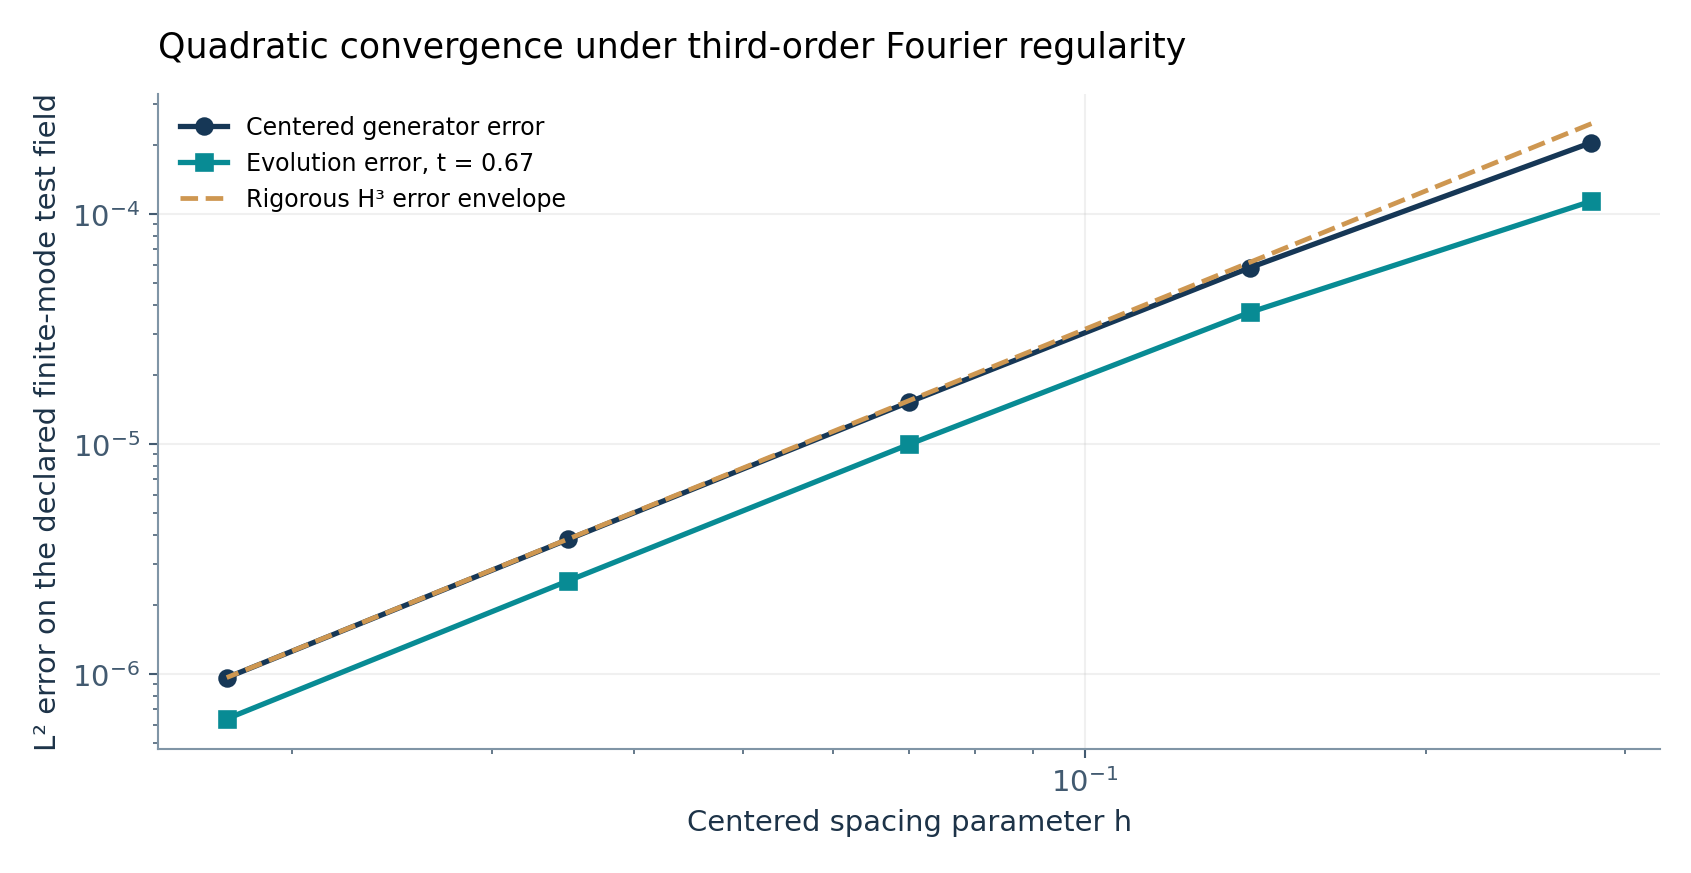
\includegraphics[width=\linewidth]{figures/block50_quadratic_convergence.png}
\caption{Finite Fourier test of the centered generator and propagator. The dashed curve is the $h^2M_3/6$ analytic envelope for the generator, rather than a fitted convergence law.}
\end{figure}

\begin{figure}[htbp]
\centering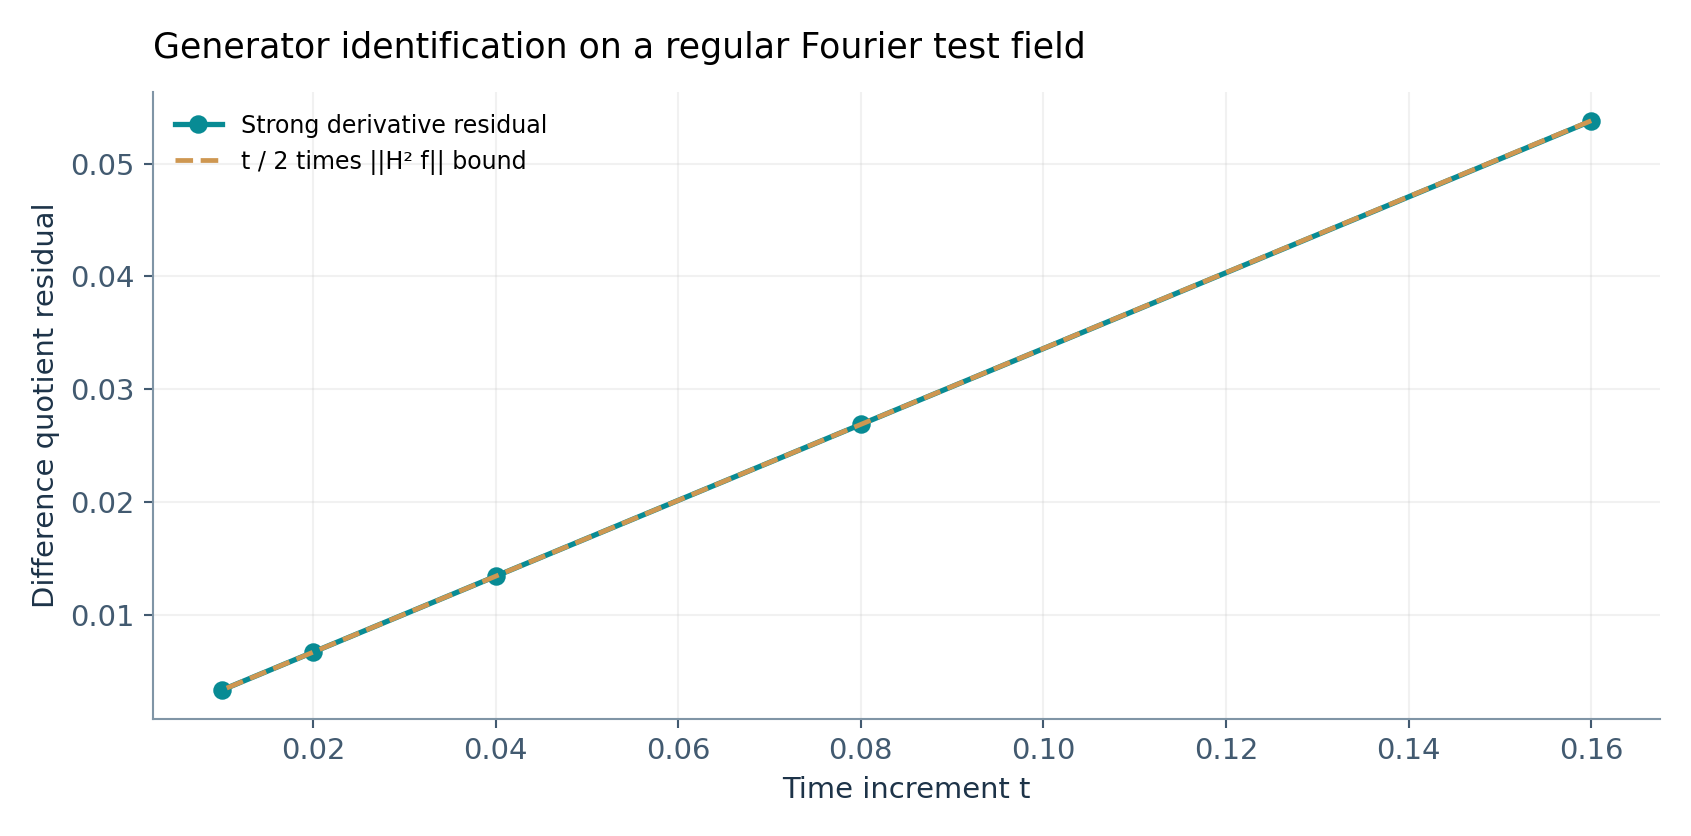
\includegraphics[width=\linewidth]{figures/block50_generator_derivative.png}
\caption{Difference quotient against $-iHf$ on the regular test field. The displayed bound is $|t|\pp{H^2f}/2$, the ordinary finite mode Taylor estimate.}
\end{figure}

The script additionally rejects a deliberate negative control: replacing $e^{-itH}$ by $e^{+itH}$ while keeping the proposed generator $-iH$ produces a difference quotient residual that approaches $2\pp{Hf}$ rather than zero. This guards the sign convention in the construction.

\section{Scope and connection to gauge transport}
The generator and resolvent arguments complete the analytic free-field construction on the fixed torus coefficient space. The strong generator, its complete domain, the physical Schrödinger equation, centered graph and resolvent limits, and third-order moment bounds have compiler-checked counterparts. The abstract spectral-functional-calculus API linkage remains separate. The technical appendix gives the exact correspondence and verification boundary.

A centered Fourier symbol on the unchanged infinite mode set is not a changing finite spatial lattice. A lattice comparison must supply sampling and interpolation, control aliasing, and prove compatibility with the chosen geometry. A background gauge coupling must also specify its operator domain and evolution. Dynamical gauge and gravitational fields impose additional equations and constraints.

The following gauge treatment begins with those local transport structures. It does not turn the free spectral result into an interacting existence theorem. The production and backreaction obstruction in the matter model is likewise unaffected by this free-field analysis.

\end{document}
